\chapter{Audience and Summary}

\marginnote[0.31in]{You will work mostly on your own laptops, but you must get familiar with the UNIX command line.  It's also important to learn how to install software and execute commands on a remote server; servers or what provide the websites you visit while browsing and they provide services to mobile apps on your phone. We've received an educational grant from Amazon to use their compute cloud called Amazon Web Services (AWS). We also have access to an IBM cluster, housed in the College of arts and sciences at USF.}

\newthought{Welcome to MSAN501}, the computational analytics boot camp at the University of San Francisco! This exercise book collects all of the labs you must complete by the end of the boot camp in order to pass.  The labs start out as very simple tasks or step-by-step recipes but then accelerate in difficulty, culminating with an interesting text analysis project. You will build all projects in Python (2.7.x).

This course is specifically designed as an introduction to analytics programming for those who are not yet skilled programmers. The course also explores many concepts from math and statistics, but in an empirical fashion rather than symbolically as one would do in a math class. Consequently, this course is also useful to programmers who'd like to strengthen their understanding of numerical methods.

\marginnote[.2in]{
\scalebox{.55}{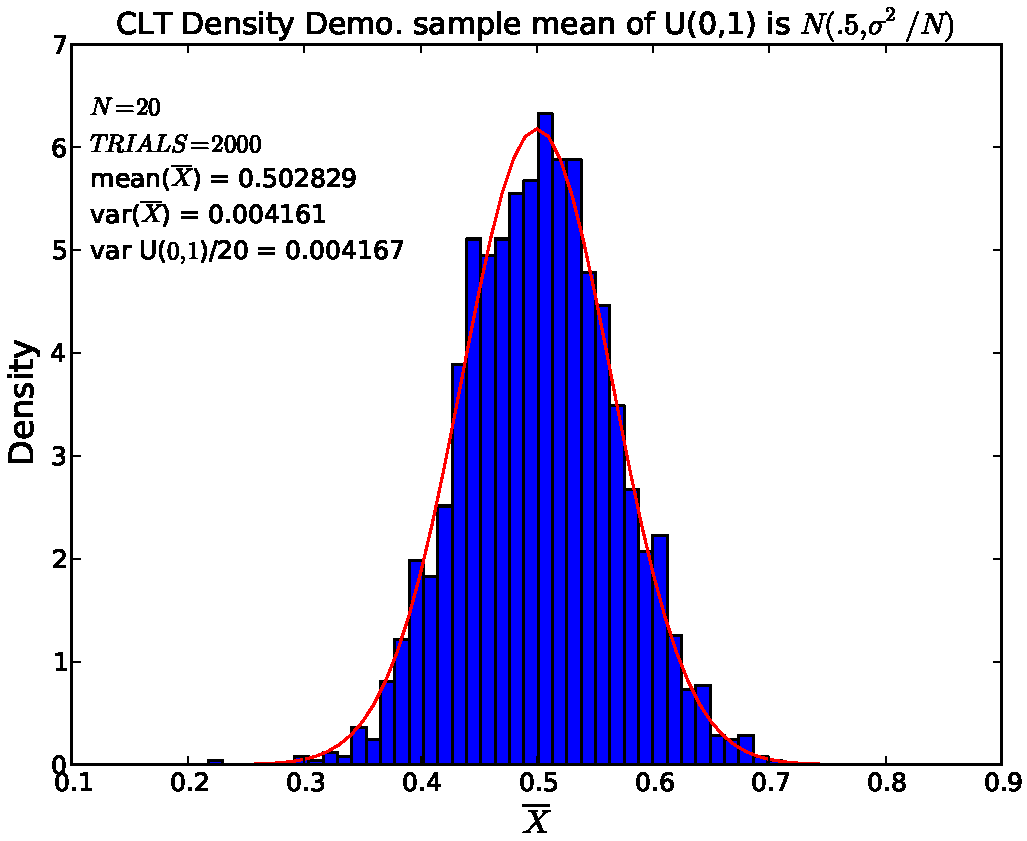
\includegraphics{figures/clt_unif-2000-20.pdf}}
\scalebox{.55}{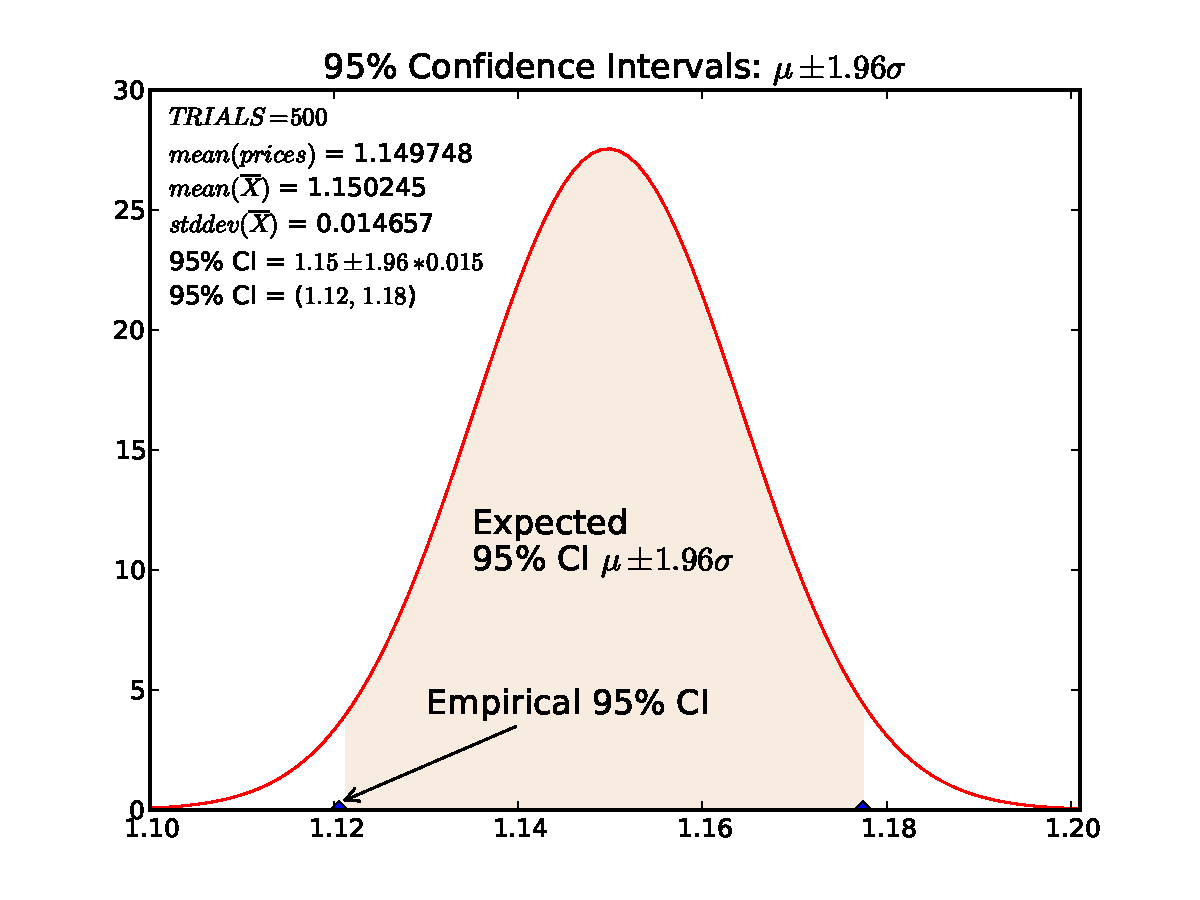
\includegraphics{figures/conf-500.pdf}}
\scalebox{.55}{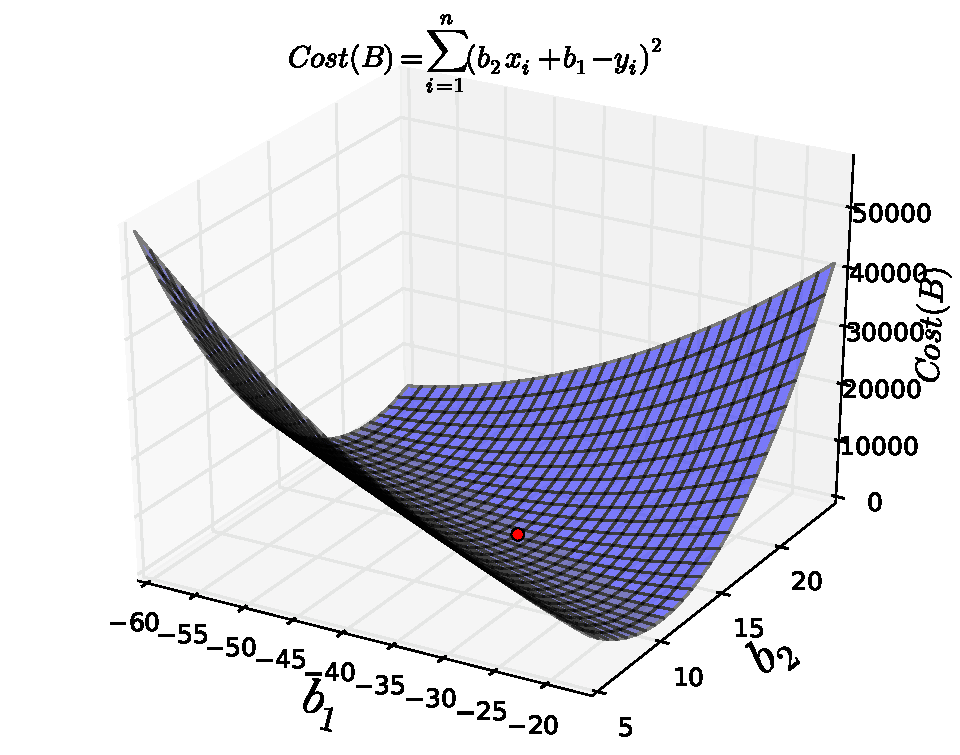
\includegraphics{figures/wage-murders-cost-3d.pdf}}
\scalebox{.55}{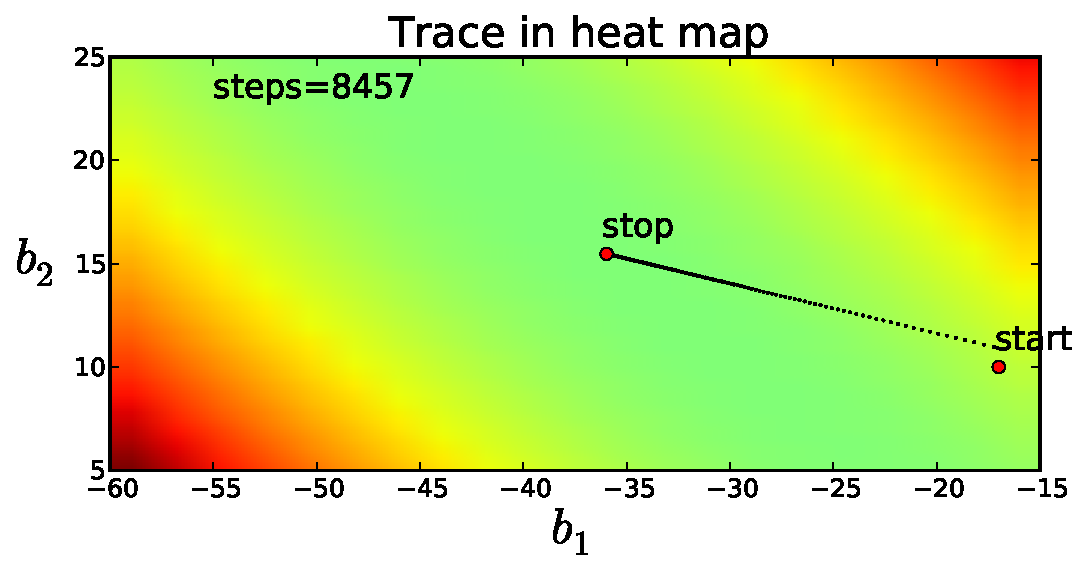
\includegraphics{figures/wage-murders-heatmap-trace1.pdf}}
}

The exercises are grouped into parts. We begin with simple programs to compute statistics, build simple data structures, and use libraries to create visualizations and then move on to learning to use the UNIX command line, launch virtual computers in the cloud, and write simple Hadoop map-reduce programs. The empirical statistics part strives to give an intuitive feel for random variables, density functions, the central limit theorem, hypothesis testing, and confidence intervals. It's one thing to learn about their formal definitions, but to get a really solid grasp of these concepts, it really helps to observe statistics in action. All of the techniques we'll use in empirical statistics rely on the ability to generate random values from a particular distribution. We can do it all from a uniform random number generator, which is the first exercise in that part.

The next set of exercises deal with function optimization. Given a particular function, $f(x)$, optimizing it generally means finding its minimum or maximum, which occur when the derivative goes flat: $f'(x) = 0$. When the function's derivative cannot be derived symbolically, we're left with a general technique called {\em gradient descent} that searches for minima. It's like putting a marble on a hilly surface and letting gravity bring it to the nearest minimum.

\marginnote{As you progress through these exercises, you'll learn a great deal about Python and the following libraries: {\tt matplotlib}, {\tt numpy}, {\tt scipy}, and {\tt py.test}.   I also recommend that you learn how to use a Python development environment called \href{http://www.jetbrains.com/pycharm/}{PyCharm}, for which we have been granted a site license.}

Finally, you'll get an introduction to text analysis. We will compute something called {\em TFIDF} that indicates how well that word distinguishes a document from other documents in a corpus.  That score is used broadly in text analytics, but our exercise uses it to summarize documents by listing the most important words.
